\documentclass{article}
\usepackage{tikz}

\begin{document}
    \begin{center}
        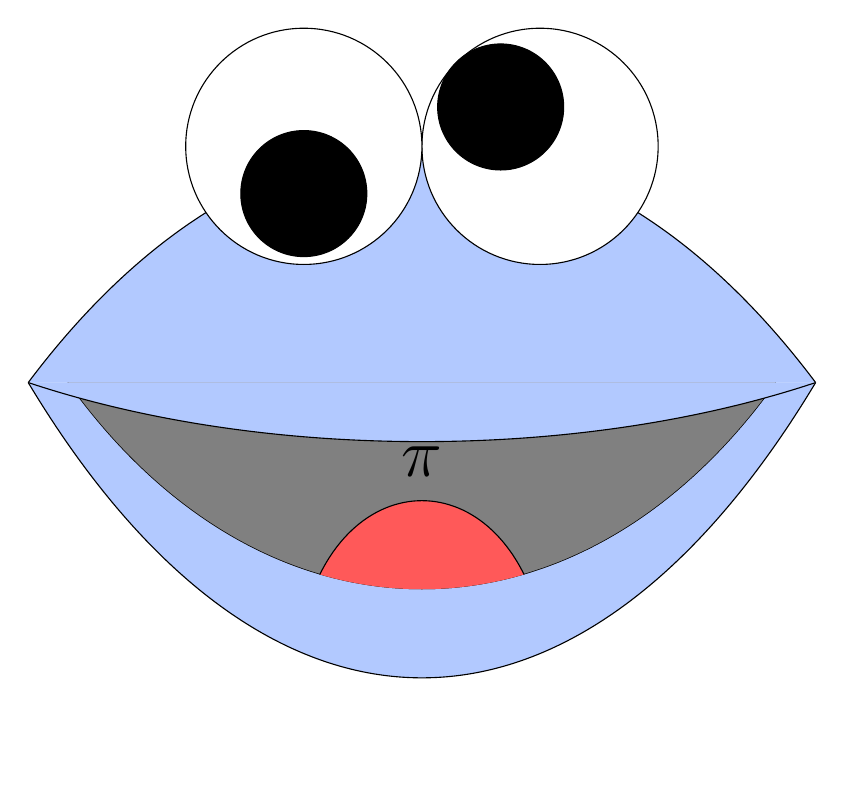
\begin{tikzpicture}
            \draw[fill=blue!70!cyan!30] (-5,0) .. controls (-2,4) and (2,4) .. (5,0);

            \draw[fill=blue!70!cyan!30] (-5,0) .. controls (-2,-5) and (2,-5) .. (5,0);
            \begin{scope}
                \clip (-4.5,0) .. controls (-2,-3.5) and (2,-3.5) .. (4.5,0);
                \draw[fill=gray] (-4.5,0) .. controls (-2,-3.5) and (2,-3.5) .. (4.5,0);
                \draw[fill=red!65] (-1.5,-3) .. controls (-1,-1) and (1,-1) .. (1.5,-3);
            \end{scope}
            \draw[fill=blue!70!cyan!30] (-5,0) .. controls (-2,-1) and (2,-1) .. (5,0);
            \draw[fill=white] (1.5,3) circle (1.5cm);
            \draw[fill=white] (-1.5,3) circle (1.5cm);
            \draw[fill=black] (1,3.5) circle (0.8cm);
            \draw[fill=black] (-1.5,2.4) circle (0.8cm);

            \node at (0,-1) [font=\Huge] {\(\pi\)};
        \end{tikzpicture}
    \end{center}
\end{document}